\documentclass{article}

\usepackage{graphicx} %package to manage images
\graphicspath{ {./images/} }

\usepackage[rightcaption]{sidecap}

\usepackage{wrapfig}

\begin{document}


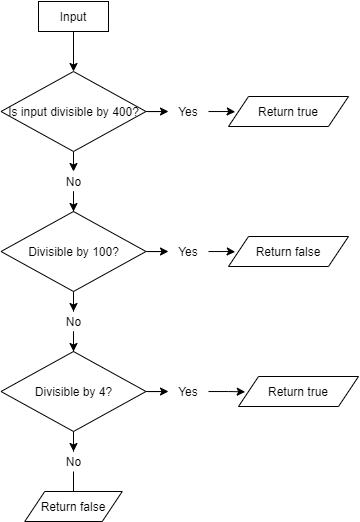
\includegraphics[scale=0.8]{Images/Diagram.png}
\\
\\
The isLeapYear method works by taking a year as an input, in the form of an integer. 
\\
First the method checks if it's divisible by 400. 
If yes, then it's a leap year. If not, then it checks if it's divisible by 100. 
If yes then it's not a leap year. If no, then it checks if it's  divisible by 4. 
If yes, then it's a leap year, if not then it's not a leap year.


\end{document}